\chapter{Konzeptioneller Entwurf}
In diesem Kapitel geht es darum die Vor- und Nachteile der unterschiedlichen
Bibliotheken anhand eines praktischen Beispieles zu zeigen. Dabei wird
\enquote{gelly-streaming} als Referenz-Implementierung benutzt. Zunächst wird
allgemein der Ablauf des Beispieles beschrieben. Dann wird die Architektur
der Referenz beschrieben. Anschließend werden die Entwürfe für die anderen
Bibliotheken beschrieben und was die Besonderheiten in Bezug auf die Referenz
sind. Abschließend werden die Probleme der Bibliotheken benannt und mögliche
Lösungsmöglichkeiten benannt.

\section{Analyse des Beispieles}
In dem Beispiel geht es darum zu überprüfen, ob ein Graph bipartite ist oder
nicht. Dies bedeutet, ob ein Graph zweifarbig färbbar ist. Um dies für einen
existierenden Graphen zu lösen, gibt es verschiedene Algorithmen. Die allgemeine
Vorgehensweise ist dabei ähnlich.

Am Beginn sind alle Knoten ungefärbt. Dann werden zwei Farben gewählt.
Anschließend wird ein Startknoten gewählt und dieser in einer der Farben markiert.
Dann werden die unmarkierten Nachbarknoten in der anderen Farbe markiert. Danach
werden deren unmarkierte Nachbarknoten wieder in der ersten Farbe markiert, usw.
bis alle Knoten markiert sind. Ein Graph ist dann bipartite, wenn alle Knoten so
markiert sind, dass keine benachbarten Knoten dieselbe Farbe haben. Diese
Vorgehensweise kann jeder selbst für kleine Graphen selbst durchführen. Je nachdem
welche Informationen über den zu überprüfenden Graphen existieren, kann der Ablauf
auch verkürzt werden. Wenn der Graph nämlich einen Kreis von ungerader Länge
enthält ist, kann der Graph nie bipartite sein unabhängig vom gewählten
Startknoten. Die Abbildung \ref{fig:bipartite-six-nodes} zeigt einen bipartiten
Graphen mit einem Kreis der Länge sechs. Während dessen die Abbildung \ref{fig:bipartite-five-nodes}
einen nicht bipartiten Graphen zeigt. Denn der Graph hat einen Kreis mit einer
ungeraden Länge und lässt sich damit nie mit zwei Farben färben egal welcher
Startknoten gewählt wurde. 

\begin{figure}
\centering
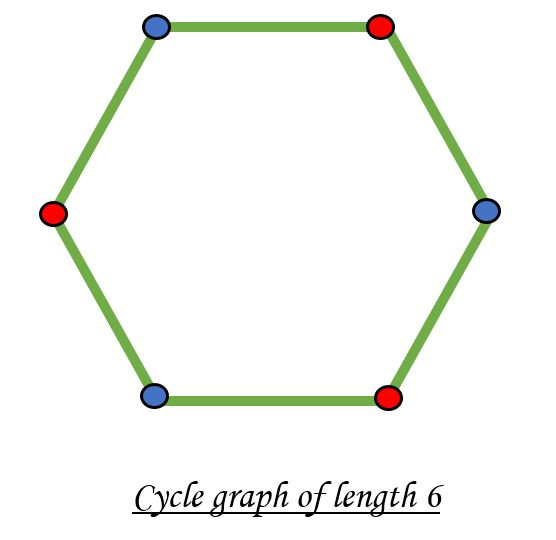
\includegraphics[scale=0.5]{../material/images/bipartite-graph-six-nodes.jpg}
\caption{bipartiter Graph mit Kreis der Länge sechs \cite{GeeksforGeeks2018}}
\label{fig:bipartite-six-nodes}
\end{figure}

\begin{figure}
\centering
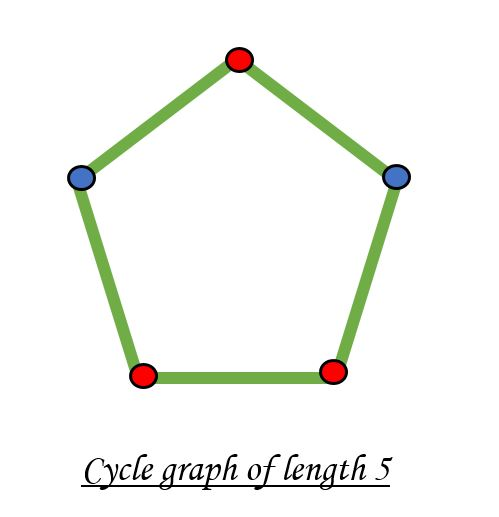
\includegraphics[scale=0.5]{../material/images/bipartite-graph-five-nodes.jpg}
\caption{nicht bipartiter Graph mit Kreis der Länge fünf \cite{GeeksforGeeks2018}}
\label{fig:bipartite-five-nodes}
\end{figure}


Wie läuft das Beispiel nun konkret ab. Zunächst werden die Daten eingelesen. Dies
erfolgt zur Vereinfachung über eine Datei. Dies kann jedoch jederzeit auf eine
alternative Eingabe umgestellt werden, zum Beispiel um die Daten von einem
Messaging-System wie Apache Kafka einlesen zu können. Dabei ist zu beachten,
dass die Bibliotheken unterschiedliche Eingabeformate unterstützen. Anschließend
werden die Daten an eine beliebige Ausgabe gesendet. Dies ist in unserem Fall die
Konsole. Wie auch schon die Eingabe kann hier natürlich auch eine andere Möglichkeit
genutzt werden.

\subsection{Architektur der Referenz-Implementierung}
Jede Streaming-Anwendung von Apache Flink wird als Job bezeichnet. Diese
Bezeichnung wird oft im Batch-Bereich benutzt. Eine Streaming-Anwendung besteht
aus zwei Teilen der Initialisierung der Streaming-Umgebung und der eigentlichen
Anwendung, welche dem EVA-Prinzip folgt. Zunächst muss die Streaming-Engine
initialisiert werden. Dabei ist es von Vorteil zu wissen, ob die spätere Anwendung
nur lokal oder remote betrieben werden soll. Lokal bedeutet in diesem Zusammenhang,
dass die Anwendung einen Apache Flink Cluster in der selbem \gls{JVM} startet.
Dies lässt sich bereits bei der Entwicklung fest einprogrammieren oder dynamisch
von Apache Flink bestimmen lassen. Die Streaming-Umgebung ist eine sehr wichtiges
Management-Objekt, welches für verschiedene Aufgaben vom Entwickler benutzt
werden sollte.

\foreigntextquote{english}[\cite{Foundation2018}]{
The LocalStreamEnvironment is a StreamExecutionEnvironment that runs the program
locally, multi-threaded, in the JVM where the environment is instantiated. It
spawns an embedded Flink cluster in the background and executes the program on
that cluster.}

Danach können die eigentlichen Daten eingelesen werden. Dazu kann ein von Apache
vordefinierter Connector zum Beispiel für Dateien benutzt werden oder eine
Bibliothek. In diesem Beispiel wird der File-Connector benutzt, welcher im Kern
von Apache Flink enthalten ist. Dieser kann einfach über die Streaming-Umgebung
aufgerufen werden. Wenn andere Connectoren zum Einsatz kommen sollen, werden
diese initialisiert und anschließend bei der Streaming-Umgebung registriert.

Die Umwandlung von Text zu Kanten muss für jede Anwendung neu definiert und
programmiert werden. Im Beispiel liegen die Daten wie schon erwähnt in einer
Datei vor. Dabei besteht jede Zeile aus genau einer Kante. Jede Kante besteht
dabei aus zwei Identifikationsnummern für die Kanten, welche durch einen
Tabulator getrennt sind. Alle Kanten sind in Apache Flink gerichtete Kanten.
Eine ungerichtete Kante kann nur erzeugt werden, wenn es eine zweite Kante gibt,
bei der die Anfangs- und End-Identifikationsnummern vertauscht sind.

\foreigntextquote{english}[\cite{Foundation2018}]{
In Gelly an Edge is always directed from the source vertex to the target vertex.
A Graph may be undirected if for every Edge it contains a matching Edge from the
target vertex to the source vertex.}

Anschließend erfolgt die Datenverarbeitung. Dabei wird auch die Ausgabe mit
definiert. Im Beispiel wird der Graph getestet, ob dieser bipartite ist. Dabei
werden die Daten in einem temporären Stream mit Fenster zwischengespeichert. Die
Überprüfung wird in eine Aggregationsfunktion eingebettet, um die
Zwischenergebnisse zu speichern. Als letztes wird der Job dann gestartet. Dabei
wird in der lokalen Umgebung dann der Cluster gestartet.

\subsection{Entwurf von \enquote{graphstream-project}}
Die Umsetzung des Beispieles ist ähnlich wie eine normale Java-Anwendung zu
programmieren. Zunächst wird die Eingabe definiert. In \enquote{graphstream-project}
werden Eingabe-Komponenten als \enquote{Sources} bezeichnet. Hier in diesem
Beispiel werden die Graph-Daten wieder von einer Datei bereitgestellt. Die
Bibliothek stellt ein Protokoll zur Datenübertragung bereit. Dadurch ist eine
einfache Kommunikation auch mit anderen Systemen möglich. Das Protokoll hat dabei
Ähnlichkeiten zum \enquote{Portable Bitmap File} Format. Beide Protokolle haben
am Anfang einen Kopf für die Meta-Informationen bevor die eigentlichen Daten
folgen. Im Unterschied zu \enquote{gelly-streaming} lassen sich die Kanten
genau spezifizieren.

\foreigntextquote{english}[\cite{Team2018}]{
ae Allows to add an edge. This command must be followed by the unique identifier
of the edge, and then the identifiers of two other nodes. As for nodes, you can
specify a parameter list. It is possible to create directed edges by adding a
“>” (greater-than) or “<” (smaller-than) character between the nodes identifiers.
This indicates the direction of the edge. When no “<” or “>” is present, the
edge is not directed.}

Die Quelle wird dann mit einer Graph-Instanz verbunden. Denn es ist möglich
den Graphen durch den Aufruf von Methoden zu ändern.

Die Implementierung von Algorithmen erfolgt bei \enquote{graphstream-project}
über das Interface Algorithm. Dieses stellt zwei Methoden bereit init und compute.
Die Methode init bekommt einen Graphen übergeben und initialisiert den Algorithmus.
Anschließend erfolgt die Manipulation des Graphen in der compute Methode.
Abschließend werden die Resultate des Algorithmus über selbst programmiert
Getter bereitgestellt. Die Ausgabe erfolgt über einen Aufruf der Konsole.

\subsection{Entwurf von \enquote{Gephi}}
Die Umsetzung des Beispieles von Gephi ist anders, als die anderen. Dort
existieren mehrere Möglichkeiten, die Aufgabenstellung zu lösen.

Die erste Möglichkeit besteht darin ein neues Statistik-Plug-In zu entwickeln
und das bestehende Streaming-Plug-In nur für die Datenübertragung zu verwenden.
Dies hätte den Vorteil, dass sehr viel von \enquote{Gephi} übernommen werden
kann und nicht in die Kommunikation eingegriffen werden muss. Der Graph muss
dabei von einem externen Service bereitgestellt werden und über HTTP übertragen.
Ob der Service die Daten selbst erzeugt oder diese zum Beispiel von einem
externen Anbieter wie Apache Kafka ausließt, hängt von den Anforderungen ab. Der
Service muss lediglich in der Lage sein, die Daten entsprechend transformieren
zu können. Die Berechnung würde dann im Programm erfolgen ebenso die Ausgabe.

Die andere Möglichkeit ergibt sich durch die direkte Benutzung des
Streaming-Plug-Ins. Das Streaming-Plugin von \enquote{Gephi} basiert wie schon
beschrieben auf HTTP. Dabei kann \enquote{Gephi} beide Seiten der
Client-Server-Verbindung repräsentieren je nach Anwendungsfall. Die
Datenübertragung erfolgt dabei standardmäßig im JSON-Format. Wenn \enquote{Gephi}
als Client betrieben wird, meldet es sich bei einem externen Service an und wartet
anschließend bis vom Service Daten gesendet werden, um diese anzuzeigen. Im
Serverbetrieb läuft \enquote{Gephi} mit einem Arbeitsbereich als Master. Dies
bedeutet, dass sich externe Services und andere \enquote{Gephi} Anwendungen am
Master anmelden können. Werden anschließend die Daten am Master durch den
Benutzer verändert oder ein Teilnehmer verändert seine eigenen Daten, dann wird
diese Information über den Master an alle Teilnehmer weitergeleitet.

Durch die beiden Seiten ergeben sich zwei mögliche Varianten bei der Benutzung
des Streaming-Plug-Ins. Die erste Variante ist es, die vorhandene \gls{API}
anzupassen. Um nicht nur den Graphen zu manipulieren, sondern auch um Statistiken
über den Graphen abfragen zu können. Die andere Variante besteht darin, einen
speziellen Event-Handler zu schreiben, der eine spezielle Funktion beim Eingang
von Ereignissen umsetzt. Da beim Eingang von Ereignissen im Standardfall nur der
Graph aktualisiert wird. Um die gewünschte Funktion umzusetzen, muss ein extra
Plug-In geschrieben werden, da einige Komponenten von der \gls{API} benötigt
werden. Das Listing \ref{code:GephiGraphHandler} zeigt den prototypischen Einsatz
eines solchen Handlers. Dieser Handler kann dann alle gewünschten Operationen
ausführen je nach Anwendungsfall. Diese Variante ist jedoch Abstraktionsebene
tiefer als, wenn der StreamingController direkt verwendet wird. Der
StreamingController erlaubt es jedoch nur Event-Handler zu registrieren, welche
auf Ereignisse reagieren können, wenn der Stream geschlossen wird.

\begin{listing}
\inputminted[breaklines=true]{java}{../material/code/GephiGraphHandler.java}
\caption{prototypischer Einsatz für einen GraphHandler}
\label{code:GephiGraphHandler}
\end{listing}

\section{Vergleich der Designs und Beschreibung der Probleme}
Eine Vergleich der verschiedenen Bibliotheken und der jeweiligen Designs ist
schwierig, da die Bibliotheken über unterschiedlichste Entwicklungsstände
verfügen und auch verschiedenen Ansätze verfolgen, wie schon in den Grundlagen
erläutert wurde.

Zunächst benutzen die Bibliotheken unterschiedliche Informationen und Darstellungen
für die Graph-Daten. Die Referenz \enquote{gelly-streaming} stellt dabei die
wenigsten Informationen bereit. Dies liegt natürlich an den verschiedenen
Konzepten der Bibliotheken. Es existieren zwei Arten von Informationen, die
eigentlichen Graph-Daten und Meta-Informationen, welche zusätzliche Informationen
zu den Graph-Daten bereitstellen. Bei \enquote{gelly-streaming} gibt es keine
Meta-Informationen und es werden lediglich die Kanten als Graph-Daten verarbeitet.
Eine Kante besteht dabei aus zwei IDs und einem Wert. Sowohl der Wert als auch
die IDs können dabei beliebige Datentypen annehmen. Es gibt lediglich eine
Einschränkung, dass beide IDs den selben Typ angehören müssen. Die Knoten werden
aus den IDs der Kanten erzeugt und haben sonst keine zusätzlichen Werte. Die
beiden anderen Bibliotheken stellen umfangreichere Daten bereit. Dort existieren
sowohl Meta-Informationen, als auch die bei \enquote{gelly-streaming} fehlenden
Knoten. Ob diese Informationen letzlich immer benötigt werden hängt natürlich
von den Anforderungen der jeweiligen Anwendung ab. Ein Entwickler könnte die
zusätzlichen Meta-Informationen mit übermitteln. Dies hat jedoch zur Folge, dass
der einzelne Wert dann immer ein komplexer Datentyp sein muss, wie zum Beispiel
eine Map, Liste,~\dots oder eine eigene Klasse.

In diesem Zusammenhang ist noch wichtig zu erwähnen, dass \enquote{gelly-streaming}
keinen weiteren Zugriff auf die Knoten, bis auf die IDs, hat im Gegensatz zu \enquote{gelly}.
Da nur Kanten eingelesen werden und Knoten automatisch aus den Ids der Kanten
erzeugt werden. Ein Entwickler ist also immer gezwungen, sich die Daten der
Knoten bei Bedarf nachzuladen. Dieses Phänomen ist auch als lazy-loading bekannt
und kommt bei Anwendungen mit Datenbanken zum tragen.

Wie schon oben erwähnt, könnte ein Entwickler die zusätzlichen Daten mit
übertragen und dann bei \enquote{gelly-streaming} die Konvertierung übernehmen.
Allerdings wird dann das nicht vorhandene Protokoll von \enquote{gelly-streaming}
zum Problem. Der Entwickler hat zwar die Freiheit beliebige Daten zu übertragen,
allerdings muss bei jedem neuen Projekt genau definiert werden, wie die zu
übertragenden Daten auszusehen haben. Dies kann gerade bei vielen Projekten zum
Problem werden. Da im Standartfall einfach eine Zeichenkette zur Verfügung steht.
Es existieren allerdings schon Ansätze diese Problematik zu lösen. Apache Flink
stellt Basisklassen für verschiedene Dateiformate bereit zum Beispiel
BinaryInputFormat, CsvInputFormat,~\dots . Damit kann ein Entwickler konkrete
Protokolle definieren bzw. gibt bei einer CSV-Datei nur die Trennzeichen an.

Die Referenz \enquote{gelly-streaming} hat Vorteile, bei der Streaming-Umgebung
und der Verteilung. Dies kommt natürlich daher, dass Apache Flink in diesen
Punkten schon über einen guten Entwicklungsstand verfügt. Darum ist
\enquote{gelly-streaming} auch die einzige Bibliothek, welche sich verteilt
betreiben lässt. Beim Vergleich der gesamten Streaming-Umgebung ist
\enquote{gelly-streaming} klar am fortschrittlichsten. Es gibt ein eigenes
Konzept für Streams, welches je nach Anforderung konfiguriert werden kann. In
unserem Beispiel soll ein einfacher Test nach Ablauf eines Zeitfensters
durchgeführt werden. Bei \enquote{gelly-streaming} wird zur Lösung dieses
Problems eine Window-Stream über den Test konfiguriert. Bei \enquote{graphstream-project}
wird ein anderer Event-System-Ansatz gewählt. Dort hat der Entwickler die
Möglichkeit zu entscheiden, ob alle Events auf einmal eingelesen werden sollen
oder nicht. Die Möglichkeit konkrete Zeitfenster zu definieren gibt es bei
\enquote{graphstream-project} nicht. Es kann lediglich abgefragt werden, ob noch
neue Events vorhanden sind. Auf die eigentlichen Events kann jedoch nicht
zugegriffen werden, sondern lediglich auf den vollständigen Graphen. Das Listing
\ref{code:GraphStreamInput} zeigt den Ablauf zum Einlesen von Events. Bei \enquote{Gephi}
kann über einen speziellen GraphEventHandler auf die Events zugegriffen werden.
Allerdings ist auch dort kein Zeitfenster vorgesehen.

\begin{listing}
\inputminted[breaklines=true]{java}{../material/code/GraphStreamInput.java}
\caption{prototypischer Ablauf zum Einlesen von Daten bei \enquote{graphstream-project}}
\label{code:GraphStreamInput}
\end{listing}

Beim Vergleich der Unterstützung von Algorithmen haben alle Bibliotheken noch
große Problem, obwohl bei \enquote{gelly-streaming} eigentlich mehr zu erwarten
wäre aufgrund der Verbindung zu Apache Flink und der Bibliothek \enquote{Gelly}.
Denn dort werden schon einige Graph-Algorithmen definiert, welche jedoch nicht in
\enquote{gelly-streaming} verwendet werden. Des Weiteren stellt \enquote{Gelly}
ein Interface GraphAlgorithm bereit, womit ein Entwickler eigene Graph-Algorithmen
entwickeln kann. Diese Möglichkeit gibt es bei \enquote{gelly-streaming} nicht.
Dies hat dort auch zur Folge, dass alle selbst definierten Algorithmen eine
Erweiterung vom SummaryAggregation sein müssen. Dies macht eine Entwicklung
neuer Algorithmen schwerer. Denn die Algorithmen bei \enquote{Gelly} werden als
Map-Reduce-Probleme beschrieben. Beim Interface GraphAlgorithm ist dies so vorgesehen,
denn dieses Interface hat nur eine run-Methode in der die konkreten
Methodenaufrufe gekapselt werden. Bei \enquote{graphstream-project} existiert
ebenfals ein Interface Algorithm für die Implementierung von Graph-Algorithmen.
Dies ist als sogenanntes Marker-Interface konzipiert. Das bedeutet, dass alle
Klassen, welche dieses Interface implementieren einen Graph-Algorithmus darstellen.
Jedoch wird dieses Interface nicht in anderen Klassen für zum Beispiel
Polymorphismus,~\dots eingesetzt. Dies lässt sich auch ganz klar an der
Interface-Struktur ablesen. Das Interface selbst besteht aus zwei Methoden.
Die init-Methode ist für die Initialisierung des Algorithmus zuständig und die
compute-Methode für die Berechnung. Die Rückgabewerte müssen über selbst
definierte Getter an den Aufrufer zurückgegeben werden. Um das Interface für
Polymorphismus nutzten zu können müsste jedoch eine Möglichkeit für die
Rückgabewerte existieren. Dies ist aber im Interface nicht vorgesehen. Um diese
Einschränkung aufzuheben, muss entweder das Interface angepasst werden um eine
Getter Methode oder die compute-Methode wird um einen Rückgabewert erweitert.
Allerdings ergibt sich dabei die Frage, was passiert, wenn mehr als ein
Rückgabewert benötigt wird.

Nachdem die Designs analysiert wurden, wird nun deren praktische Umsetzung
beschrieben und welche Problem dabei auftraten.
